\section{Experiments and Results}

We show the speedup obtained using our improved heuristics against the
conventional heuristics for Simulated Annealing as prescribed
by~\cite{hors06}. We also compare the results we obtain against the
K-way graph partitioning algorithm~\cite{gkar95} and heterogeneous bin
packing heuristic~\cite{mmar11}.

\subsection{K-way graph partitioning}
\label{sec:k-way-graph}

Graph partitioning plays an important role in the multi-processor and
VLIW scheduling and partitioning
algorithms~\cite{aale01,kpur99,enys98}. K-way graph partitioning is an
important algorithm, which partitions a given graph into K or less
parts, resulting in load balanced allocations. K-way partitioning mixed
with min-edge cuts can form a good tool to partition a task-graph onto a
multi-processor system, resulting in equal utilization of PEs and
reduced communication costs. We have utilized the Metis~\cite{gkar95}
graph partitioning tool to perform a K-way graph partitioning onto
heterogeneous multi-processor architectures for comparison
purposes.

Metis is a graph partitioner, which implements K-way partitioning with
min-edge cut as the primary objective. The weights on the graph nodes
are represented as constraints. Each graph node can have multiple-node
weights, representing different criteria. The edges between nodes can be
weighted themselves, but as opposed to nodes, edges can only be
decorated with a single weight. Moreover, the unique point about Metis
is that one can use a concept called ``tp-weights'', which give
weightage, to different node constraints when performing load-balancing
during K-way graph partitioning. These are the only features of Metis
that we required when implementing our algorithm. Metis provides a
number of other features, which the readers can lookup in~\cite{gkar95}.

The gist of our K-way task partitioning approach onto a heterogeneous
multi-core architecture is as follows:

\begin{itemize}

\item Our resource graph is first described as a simple graph in
  metis. In this description each of the two capabilities $W^i_0$ and
  $W^i_1$ are described as two constraints for each node in the
  graph. The communication bandwidth is described as edge weights in
  metis.

\item Once we have the resource graph in the metis format we calculate
  the tp-weights. There are two tp-weights generated, one for each of
  the resource node capabilities. Let us revisit the 4 $\times$ 4 mesh
  shown in Figure~\ref{fig:1r}. For each processor the MIPS tp-weight is
  calculated by the formula: $W^i_0/\sum_{\forall i \in
    V_r}(W^i_0)$. Similarly, we can easily calculate the tp-weight
  metric for each PEs vector length capability as: $W^i_1/\sum_{\forall
    i \in V_r}(W^i_1)$. These fractions give a relative approximation of
  the capabilities of each PE compared to the other.

\item The nodes in our task graph are described as node in the metis
  format. The two requirements ($R^i_0$ and $R^i_1$) for each task node
  are described as two constraints in the metis node format. The edge
  weights in our task graph are described as edge weights in the metis
  graph format.

\item Once we have the task graph described in the metis format along
  with the tp-weight metric for each PE in the resource graph. We ask
  for a $|V_r|$ partition from metis, giving the tp-weight metric for
  each constraint of the task graph.

\item The resultant partition is then used to calculate the objective in
  Equation~(\ref{eq:2}).

\end{itemize}


\subsection{Heterogeneous bin packing heuristic}
\label{sec:heter-bin-pack}

Heuristic bin packing solutions have given good results in the general
case~\cite{ecof78}. Comparing with the heterogeneous bin packing
heuristic~\cite{mmar11} allows us to gauge the effectiveness of our
algorithm against a standard technique.

Let $\mathcal{I}$ be the items to be accommodated into the bins and let
$\mathcal{K}$ be the set of bins available.  From the standpoint of the
mapping problem, $\mathcal{I}$ refers to the set of task graph nodes
($|V_t|$) and $\mathcal{K}$ refers to the nodes in the resource graph
($|V_r|$). Similar to the Knapsack problem~\cite{sski08}, by which A-BFD
is inspired, each element $i \in \mathcal{I},\ \mathcal{K}$ has two
constraints on them represented by $c_i$ (cost), which translates to the
PE capability $W^i_0$ and $V_i$ (volume), which translates to the
capability $W^i_1$, respectively.
% Right off the bat, this seems to be a significant advantage, our
% framework has over heterogeneous bin packing, as \textit{A-BFD} only
% works with two constraints whereas our framework poses no such
% restrictions.
\textit{A-BFD} proceeds to sort $\mathcal{I}$ according
to non-increasing order of their volume and sorts $\mathcal{K}$
according to non-increasing order of the ratio $c_i/V_i$. Then, it
proceeds to allocate items from $\mathcal{I}$ into best bins $b \in
\mathcal{S}$. A ``best" bin, i.e., the bin with maximum free space, is
defined as the bin volume minus the sum of volumes of the items loaded
into it. % In the mapping problem setting, this becomes a double edged
% sword as it boils down to a single constraint solving problem giving
% higher priority to the second constraint (vector requirement of the
% application-tasks $w^t_1(i)$ and vector capability of the resources
% $W^r_1(i)$).

The post pass in \textit{A-BFD} chooses every bin that has atleast one
item allocated to it and tries to find an empty bin, that has a higher
or equal volume than the allocated volume on the chosen bin but also has
a lower cost. If it finds such an empty bin, then it transfers all the
items allocated to the chosen bin to the newly found empty bin which is
cheaper. One of the main advantages of \textit{A-BFD} is that it is very
fast with a best case complexity of $O(N_\mathcal{I})$ without the post
pass, where $N_\mathcal{I}$ is the number of items (number of tasks
$|V_t|$ in the application graph $G_t$). Including the post pass, the
best case complexity becomes $O(N_\mathcal{I} + N_\mathcal{K})$ where
$N_\mathcal{K}$ is the number of bins (number of PEs $|V_R|$ in the
resource graph $G_r$).


\subsection{The experimental setup}
\label{sec:experimental-setup}

We need to setup the resource graph and the task graph for experimental
purposes. Herein, we describe our setup for both.

\subsubsection{The resource graph setup}
\label{sec:resource-graph-setup}

The experimental section consist of the following:

\begin{enumerate}

\item An multi-core system with \numtplgynodes nodes. A node could be
  just a multi-core CPU or a multi-core CPU with a GPU attached to
  it. \numtplgynodes varies in a normal distribution from 2 to 16.

\item The bandwidth is selected from a set \mbox{$\bwset = \{B_1, B_2, ...,
  B_{|\bwset|}\}$}. Every communication link weight ($W^c$) is selected
from the set \bwset. The elements of the set \bwset varies in the normal
distribution: 10Mb/s to 1Gb/s, representative of the multi-core
connection networks in today's machines.

\item A set of \gpunum GPUs where \gpunum is at most \numtplgynodes. The
  GPUs are connected in the network at pre-determined locations, chosen
  randomly in the normal distribution of 25\% to 75\% of $|V_r|$.

\item A set $\veclenset = \{V_1, V_2, V_3, ... V_{|\veclenset|}\}$ where
  $V_i$ is a power of 2.  Every GPU in this experiment has a vector
  length of $V_i$ where $V_i$ is sampled randomly from the set
  \veclenset. The elements of set \veclenset are chosen from a normal
  distribution ranging from 1024 to 16284.

\item A set $\corenumset = \{C_1, C_2, C_3, ... C_{|\corenumset|}\}$
  where $C_i$ is a power of 2.  Every CPU in this experiment has $C_i$
  cores where $C_i$ is sampled randomly from the set \corenumset.

\item A set $\mipsset = \{M_1, M_2, M_3, ... M_{|\mipsset|}\}$ where
  $M_i$ is a power of 2.  Every $C_i \in \corenumset$ and GPU in this
  experiment has a MIPS count of $M_i$ where $M_i$ is sampled randomly
  from the set \mipsset. The elements of set \mipsset are chosen from a
  normal distribution ranging from 100 to 1000000.

\end{enumerate}

For given values of \numtplgynodes, \gpunum, \veclenset, \corenumset,
and \mipsset and a given application, let the $k$-th \ul{trial} be
defined as one execution of the following sequence of steps.

\begin{itemize}

\item For each GPU $G_i$, sample \veclenset and \mipsset randomly to
  determine its vector length $V_i$ and MIPS count $M_i$. \label{i1}

\item For each CPU $P_i$, sample \corenumset randomly to determine the
  number of cores $C_i$ in the processor $P_i$.~\label{i2}

\item For each core $C_i$ in the processor $P_i$ sample $V_i$ and $M_i$
  randomly from set \veclenset and \mipsset.

\item Use our framework to extract data and task parallelism that is
  best utilizable by the heterogeneity created by parameters in items 1,
  2, and 3 above. Determine the execution time
  $Latency^{\zeta_\mathcal{M}}$.

\end{itemize}

An experiment, \expt(\numtplgynodes, \gpunum, \veclenset, \corenumset
\mipsset), consists of conducting enough of the above trials so that
width of the 95\% confidence interval on the average value of
$Latency^{\zeta_\mathcal{M}}$ is less than 10\% of the average
value. This results in a variable number of trials with different
experimental setups. Note that two trials differ from each other only in
the seed for the random number generator.  This reduces the dependence
of our results on a lucky sequence of numbers from the random number
generator.

\subsubsection{The task graph setup}
\label{sec:task-graph-setup}

We chose 5 applications: binomial option pricing (a financial
derivatives application), 2-dimensional convolution (for image
processing), gram Schmidt linear algebra kernel, 2-dimensional
Gauss-seildel stencil computations, and finally our motivating example
itself the 2-dimensional Jacobi stencil computation. Next for these 5
applications, we varied the vector strip from 10 to 50, which resulted
in graphs varying from around 50 to 5000 nodes and with 23 to 12,000
edges. For example, given a task node with a vector length requirement
($w^i_1$) of 30,000 elements, a vector strip of 10 means dividing the
total vector requirement by 10, which results in 10 nodes each requiring
3000 vector elements. Similarly, the instruction count ($w^i_0$) for
each node varies depending upon the application at hand.

A detailed description of the applications and their features is shown
in Table~\ref{tab:1}. In general the vector requirement of the
applications in our benchmark suite varies from 1000 to 1 Million
elements. The instruction count varies from around 1 to 0.3 billion. The
edge weights depicting the amount of data transfer on the other hand
varies from 3000 bytes to almost 4.8 Mega byte.

\begin{table}[h!]
  \centering
  \begin{tabular}{|c|c|c|c|}
    \hline
    \textbf{Application} & \textbf{Vector strip} & $|V_t|$ & $|E_t|$ \\
    \hline
    \multirow{5}{*}{Binomial option pricing} & 10 & 82 & 206 \\
    & 20 & 102 & 306 \\
    & 30 & 122 & 406 \\
    & 40 & 142 & 506 \\
    & 50 & 162 & 606 \\
    \hline
    \multirow{5}{*}{Convolution} & 10 & 79 & 143 \\
    & 20 & 89 & 173 \\
    & 30 & 99 & 203 \\
    & 40 & 109 & 233 \\
    & 50 & 119 & 263 \\
    \hline
    \multirow{5}{*}{Gram Schmidt} & 10 & 228 & 443 \\
    & 20 & 838 & 1653 \\
    & 30 & 1848 & 3663 \\
    & 40 & 3258 & 6473 \\
    & 50 & 5068 & 10083\\
    \hline
    \multirow{5}{*}{Gauss-Seidel} & 10 & 227 & 531 \\
    & 20 & 837 & 2041 \\
    & 30 & 1847 & 4551 \\
    & 40 & 3257 & 8061 \\
    & 50 & 5067 & 12571\\
    \hline
    \multirow{5}{*}{Jacobi} & 10 & 48 & 130 \\
    & 20 & 78 & 240 \\
    & 30 & 108 & 350 \\
    & 40 & 138 & 460 \\
    & 50 & 168 & 570\\
    \hline
  \end{tabular}
  \caption{The task graph setup}
  \label{tab:1}
\end{table}

\subsection{The results}
\label{sec:results}

The comparison of our simulated annealing approach with other techniques
are described in the next sub sections. In all the upcoming comparisons
we set the value of $q=0.75$ in our SA and standard SA techniques. This
value of $q$ is a good compromise between a slow running SA heuristic vs
application latencies, since a bigger value of $q$, results in larger
explored state space. For the aforementioned experimental setup our and
standard SA techniques were run for 10 minutes.

\subsubsection{Comparison with K-way partitioning}
\label{sec:comparison-with-k}

The results comparing K-way graph partitioning with our SA heuristic is
shown in Figure~\ref{fig:metis}. The 3D surface graphs shown in
Figure~\ref{fig:metis} consist of two surfaces. Each surface plots the
execution latency of the application, in $log_{10}(sec)$ scale, on the
Z-axis. The X and Y axes show the number of PEs in the underlying
architecture and the vector strip sizes, respectively.

The surface produced by the K-way partitioning heuristic is above the
surface created by our SA heuristic for all applications, other than
convolution and Jacobi. The major statistics comparing the two
approaches is provided in Table~\ref{tab:2}. In Table~\ref{tab:2}, The
\textbf{Max latency} and the \textbf{Min latency} columns, provide the
maximum and minimum latencies observed in Figure~\ref{fig:metis} for
each of the applications. The last column (\textbf{Better (\%)}) gives
the number of points in the surfaces that were better in our SA
technique compared to K-way graph partitioning.

\begin{figure*}[t!]
  \centering
  \subfigure[Binomial Option Pricing]{
    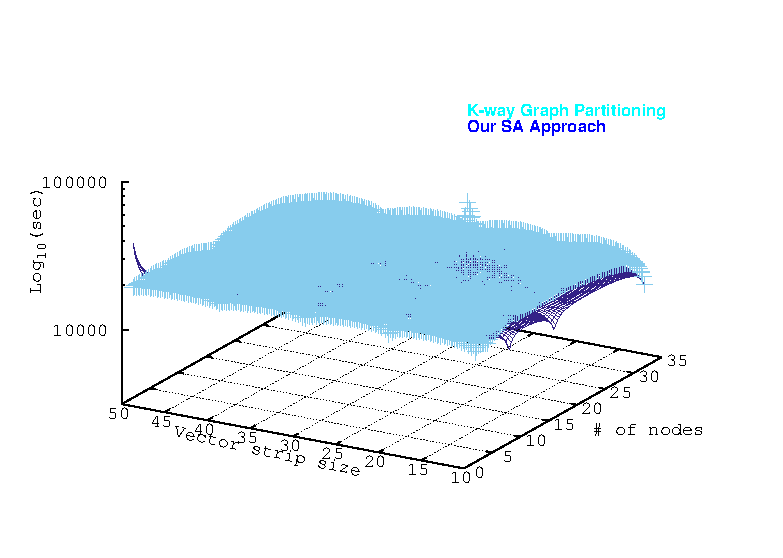
\includegraphics[angle=0, scale=0.32]{./figures/bin_metis_surface}
    \label{fig:bin1metis}
  }
  \subfigure[2 Dimensional Convolution]{
    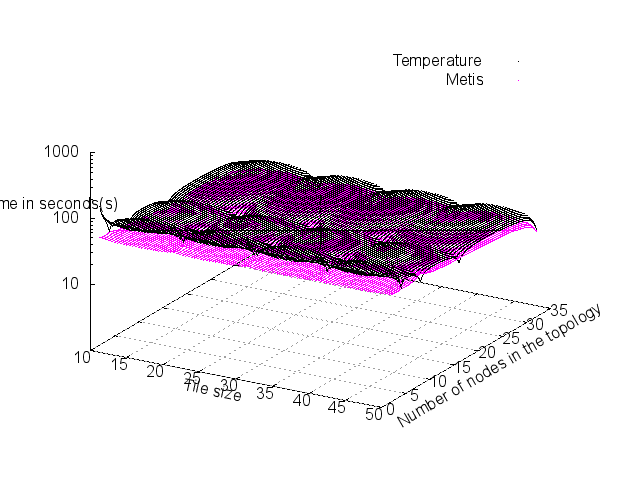
\includegraphics[angle=0, scale=0.32]{./figures/conv_metis_surface}
    \label{fig:conv1metis}
  }
  \subfigure[Gram schmidtt linear-algebra kernel]{
    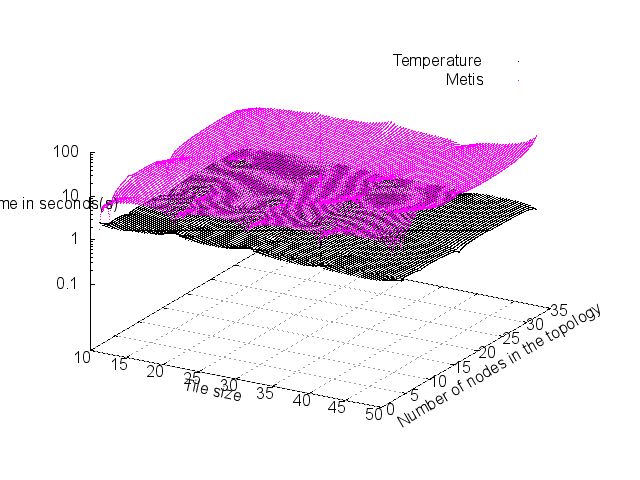
\includegraphics[angle=0, scale=0.32]{./figures/gram_metis_surface}
    \label{fig:gram1metis}
  }
  \subfigure[2 Dimensional Seidel stencil computation]{
    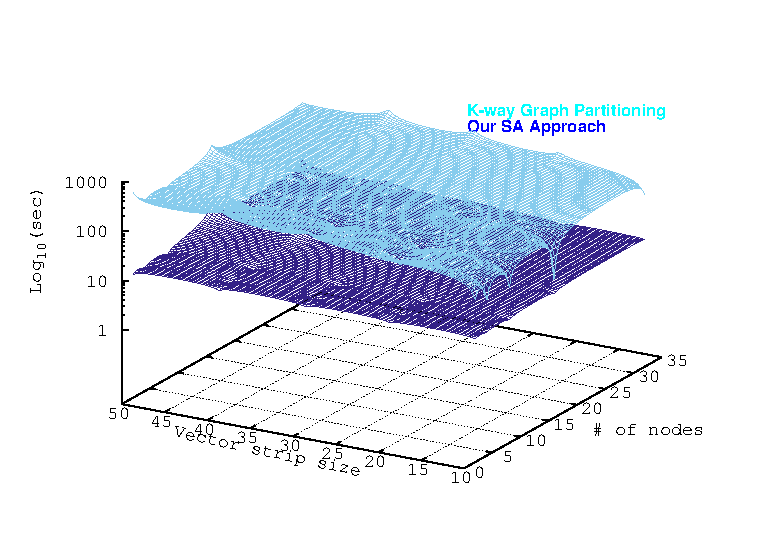
\includegraphics[angle=0, scale=0.32]{./figures/sei_metis_surface}
    \label{fig:sei1metis}
  }
  \subfigure[2 Dimensional Jacobi stencil computation]{
    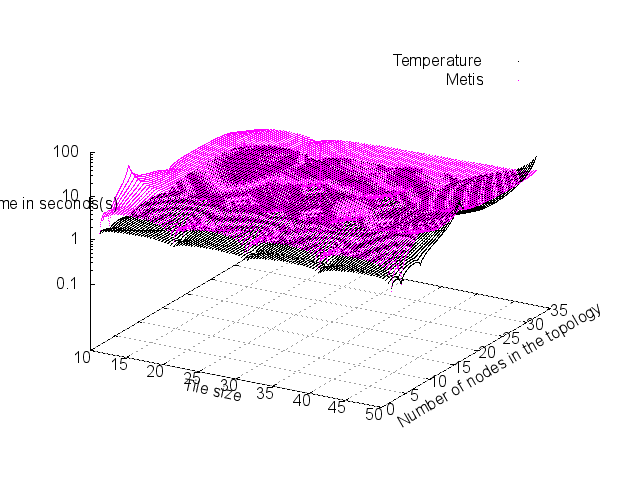
\includegraphics[angle=0, scale=0.32]{./figures/jac_metis_surface}
    \label{fig:jacl1metis}
  }
  \caption{Comparison of application latencies: Our SA approach Vs K-way
  graph partitioning}
  \label{fig:metis}
\end{figure*}

\begin{table*}[t!]
  \centering
  \begin{tabular}{|c|c|c|c|c|c|}
    \hline
    \textbf{Application} &
    \multicolumn{2}{|c|}{\textbf{Max latency (sec)}} &
    \multicolumn{2}{|c|}{\textbf{Min latency (sec)}} &
    \textbf{Better (\%)} \\
    \hline
    & {K-way} & {Our SA approach} &
    {K-way} & {Our SA approach} & K-way vs Our SA approach\\
    \hline
    Binomial option pricing & 79947.2 & 53404.8 & 11218.1 & 10975.5 & 94 \\
    \hline
    Convolution & 52.85 & 124.309 & 19.64 & 19.64 & 12\\
    \hline
    Gram Schmidt & 54.13 & 2.96 & 1.33 & 0.91 & 64\\
    \hline
    Gauss-Seidel & 542.44 & 32.99 & 9.67 & 9.67 & 68\\
    \hline
    Jacobi & 16 & 14.69 & 0.95 & 0.89 & 32\\
    \hline
  \end{tabular}
  \caption{Major statistics comparing K-way graph partitioning and our
    SA approach}
  \label{tab:2}
\end{table*}


\subsubsection{Comparison with heterogeneous bin packing heuristic}
\label{sec:comp-with-heter}

Comparison of our SA technique with heterogeneous bin packing heuristic
is shown in Figure~\ref{fig:ho}. Unlike, K-way graph partitioning, the
bin packing heuristic could not partition the binomial option pricing
and Gauss-Seidel examples for any vector strip size, because the bin
packing algorithm gives up if there is no underlying PE that can support
the required vector tile size. Our SA heuristic on the other hand runs a
part of the vector on the underlying PE and then iterates in a loop
until all vector computations are finished. For example, if the task
graph requires a 1000 vector elements that need to be processed at once,
and the largest vector capability in the resource graph is a 100 then,
our heuristic will allocate a 100 vector elements onto the underlying
hardware and then increase the instruction count by 10.

The heterogeneous bin packing heuristic performs much worse compared to
our approach. This can be blamed onto the fact that heterogeneous bin
packing prioritizes vector length over number of instruction
count. Heterogeneous bin packing packs a large number of vectors nodes
from the application graph into a single large vector PE, including
those task nodes, which have a very small vector count ($w^i_0$), but a
very large instruction count ($w^i_1$). The major facts about
Figure~\ref{fig:ho} are highlighted in Table~\ref{tab:3}.

\begin{figure*}[t!]
  \centering
  \subfigure[2 Dimensional Convolution]{
    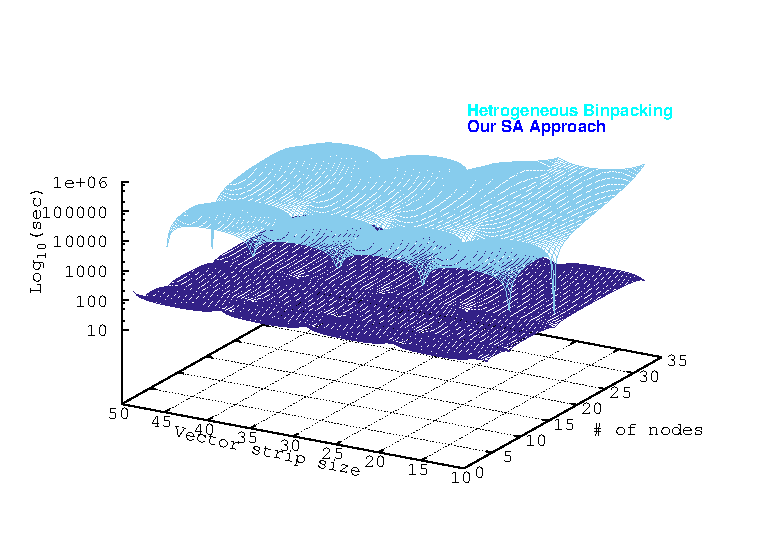
\includegraphics[angle=0, scale=0.32]{./figures/conv_hbp_surface}
    \label{fig:conv1ho}
  }
  \subfigure[Gram schmidtt linear-algebra kernel]{
    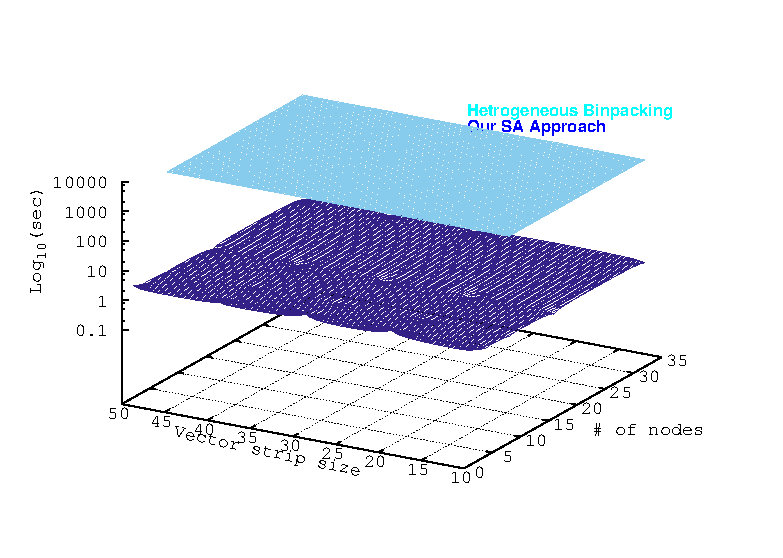
\includegraphics[angle=0, scale=0.32]{./figures/gram_hbp_surface}
    \label{fig:gram1ho}
  }
  \subfigure[2 Dimensional Jacobi stencil computation]{
    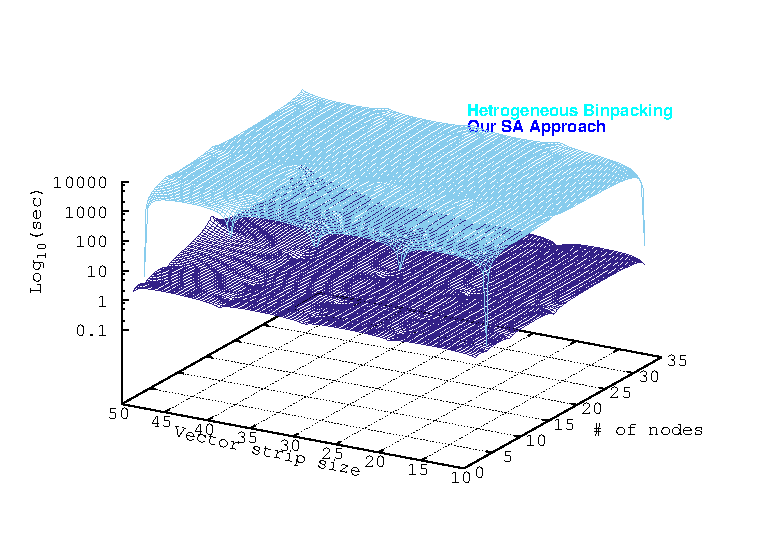
\includegraphics[angle=0, scale=0.32]{./figures/jac_hbp_surface}
    \label{fig:jacl1ho}
  }
  \caption{Comparison of execution times of ``Our Framework" and
    ``Heterogeneous Bin Packing"}
  \label{fig:ho}
\end{figure*}

\begin{table*}[t!]
  \centering
  \begin{tabular}{|c|c|c|c|c|c|}
    \hline
    \textbf{Application} &
    \multicolumn{2}{|c|}{\textbf{Max latency (sec)}} &
    \multicolumn{2}{|c|}{\textbf{Min latency (sec)}} &
    \textbf{Better (\%)} \\
    \hline
    & {HBP} & {Our SA approach} &
    {HBP} & {Our SA approach} & HBP vs Our SA approach\\
    \hline
    Convolution & 489065 & 78.52 & 53.64 & 16.26 & 94\\
    \hline
    Gram Schmidt & 18984.5 & 177.97 & 2947.65 & 1.20 & 94\\
    \hline
    Jacobi & 13919.2 & 39.89 & 1.69 & 0.97 & 92\\
    \hline
  \end{tabular}
  \caption{Major statistics comparing heterogeneous bin packing and our
    SA approach}
  \label{tab:3}
\end{table*}

\subsubsection{Comparison with established SA}
\label{sec:comp-with-establ}

The figures showing the comparison of our approach with the established
SA approach of~\cite{hors06} is shown in Figure~\ref{fig:stdsa}. There
is not a single case where our SA approach is worse than the current
established technique. The major statistics comparing the two techniques
for Figure~\ref{fig:stdsa} are shown in Table~\ref{tab:4}.

ARAVIND: REASONS??

\begin{figure*}[t!]
  \centering
  \subfigure[Binomial Option Pricing]{
    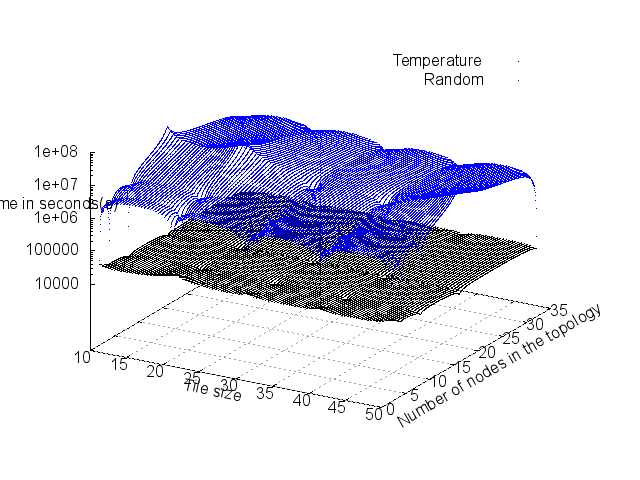
\includegraphics[angle=0, scale=0.32]{./figures/bin_random_surface}
    \label{fig:bin1random}
  }
  \subfigure[2 Dimensional Convolution]{
    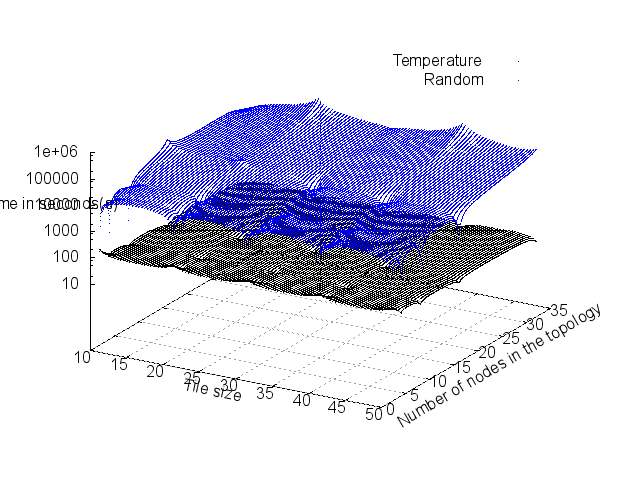
\includegraphics[angle=0, scale=0.32]{./figures/conv_random_surface}
    \label{fig:conv1random}
  }
  \subfigure[Gram schmidtt linear-algebra kernel]{
    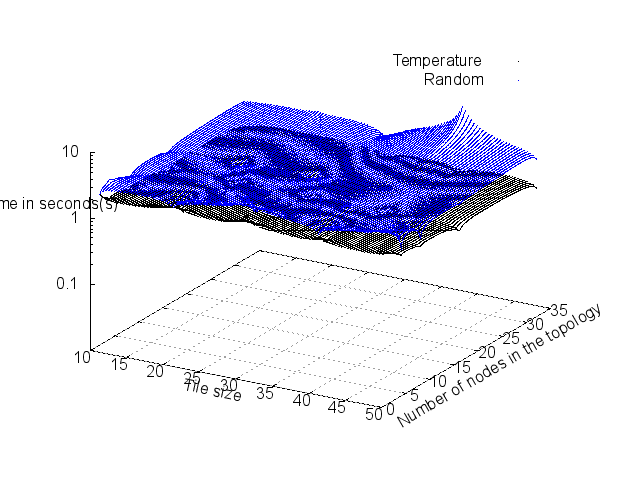
\includegraphics[angle=0, scale=0.32]{./figures/gram_random_surface}
    \label{fig:gram1random}
  }
  \subfigure[2 Dimensional Seidel stencil computation]{
    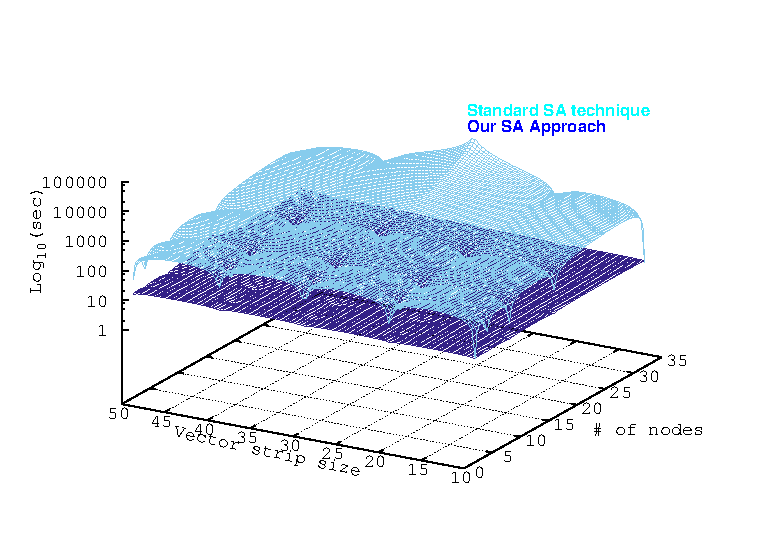
\includegraphics[angle=0, scale=0.32]{./figures/sei_random_surface}
    \label{fig:sei1random}
  }
  \subfigure[2 Dimensional Jacobi stencil computation]{
    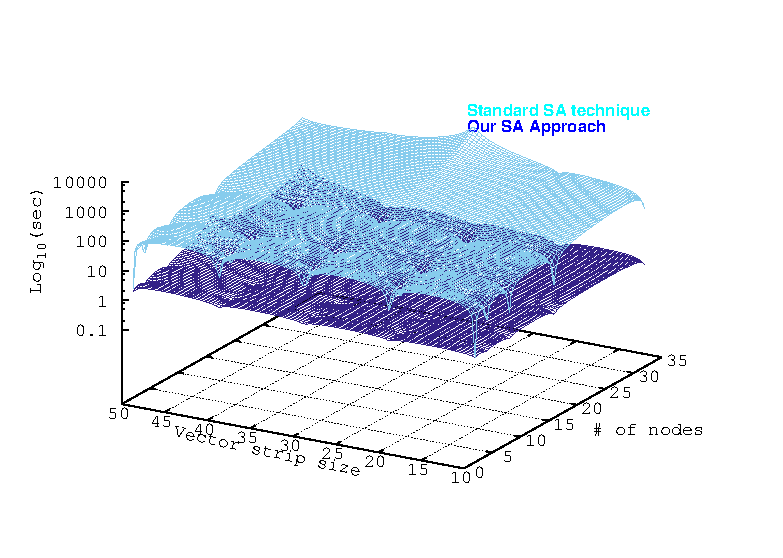
\includegraphics[angle=0, scale=0.32]{./figures/jac_random_surface}
    \label{fig:jacl1random}
  }
  \caption{Comparison of application latencies: Our SA approach Vs
    standard SA approach}
  \label{fig:stdsa}
\end{figure*}

\begin{table*}[t!]
  \centering
  \begin{tabular}{|c|c|c|c|c|c|}
    \hline
    \textbf{Application} &
    \multicolumn{2}{|c|}{\textbf{Max latency (sec)}} &
    \multicolumn{2}{|c|}{\textbf{Min latency (sec)}} &
    \textbf{Better (\%)} \\
    \hline
    & {Standard SA} & {Our SA} &
    {Standard SA} & {Our SA} & Standard SA vs Our SA\\
    \hline
    Binomial option pricing & 219230 & 53404.8 & 25967.5 & 8971 & 95 \\
    \hline
    Convolution & 220525 & 124.31 & 50.34 & 19.64 & 76\\
    \hline
    Gram Schmidt & 10.04 & 2.96 & 0.96 & 0.91 & 92\\
    \hline
    Gauss-Seidel & 14607.8 & 32.99 & 9.07 & 9.67 & 72\\
    \hline
    Jacobi & 3504.44 & 14.69 & 0.95 & 0.89 & 88\\
    \hline
  \end{tabular}
  \caption{Major statistics comparing standard SA and our SA heuristics}
  \label{tab:4}
\end{table*}

\subsubsection{Effect of varying temperature}
\label{sec:varying-temperature}




%%% Local Variables: 
%%% mode: latex
%%% TeX-master: "bare_conf"
%%% End: 
